\section{Marco teórico}

\subsection{Eliminación Gaussiana}

Los sistemas de ecuaciones lineales pueden ser representados en forma matricial como \textit{Ax=b}, donde A representa la matriz de los coeficientes que acompañan a cada una de las incógnitas, \textit{x} representa al vector de incógnitas y \textit{b} al vector de términos independientes. Para los sistemas cuadrados, donde hay misma cantidad de incógnitas que de ecuaciones, el método de eliminación Gaussiana busca darle valor a los coeficientes del vector de incógnitas y resolver el sistema lineal. El modelado de sistemas de ecuaciones con matrices se extiende a una amplia gama de disciplinas como los gráficos por computadora, las finanzas, las ingenierías, entre otras, no serían como las conocemos sin este objeto y las operaciones que podemos hacer con él. 

\begin{figure}[h]
    \centering
    \begin{minipage}{0.3\linewidth}
        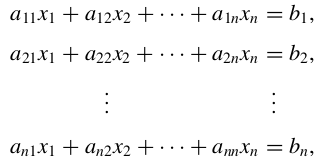
\includegraphics[width=\linewidth]{img/sistema_de_ecuaciones.png}
        \caption{Un sistema de ecuaciones}
    \end{minipage}
  \begin{minipage}{0.45\linewidth}
      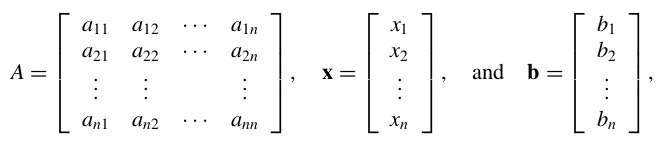
\includegraphics[width=\linewidth]{img/combinacion_lineal.png}
      \caption{Su forma matricial}
  \end{minipage}
  \caption{Sistemas de ecuaciones con su respectiva representación matricial}
\end{figure}

El proceso para resolver mediante este método comienza con la matriz original y se va aplicando sobre ella una serie de pasos hasta obtener una forma triangular superior. Para realizar esto, se recorre cada elemento perteneciente a la diagonal principal $a_{ii}$ poniendo en ceros los elementos inferiores a éste. Este proceso se llama diagonalización. Una vez diagonalizado el sistema, buscamos darle valores a los coeficientes del vector de incógnitas por medio de un despeje desde abajo hacia arriba, o sea, empezamos por el coeficiente inferior del vector $x$ y subiendo por el mismo usando los valores despejados previamente para obtener nuevas soluciones para los próximos coeficientes. El método descripto se conoce como \textit{Gaussian elimination with Backward substitution} \cite{Burden11}. Este método para resolver el sistema de ecuaciones tiene una complejidad computacional de $\mathcal{O}(n^3)$.

\subsection{Métodos de pivoteo para diagonalización}

Para casos donde encontramos, o por medio del mismo proceso de diagonalización nos "creamos", un cero en la diagonal de la matriz existen formas de obtener versiones equivalentes del sistema donde podemos continuar nuestro algoritmo de eliminación Gaussiana. Estos métodos se llaman \textit{pivoteos parciales o totales} y constan en hacer intercambios de filas o de columnas para que el sistema se pueda seguir soportando el algoritmo. Cuando los intercambios son de filas los llamamos pivoteos parciales y cuando lo son de filas y columnas los llamamos pivoteo total. En el presente trabajo nos centraremos en pivoteos parciales. Observese en la figura \ref{fig:pivoting} como el proceso de eliminación gaussiana puede solucionar el hecho de encontrar un cero en la diagonal por medio del intercambio de filas.

\begin{figure}
    $$
    \left[\begin{array}{cccc|c}
    2 & 2 & -1 & 3 & 13 \\
    -2 & -2 & 0 & 0 & -2 \\
    4 & -1 & -2 & 4 & 24 \\
    -6 & -2 & 2 & -3 & -10
    \end{array}\right] \rightarrow \begin{gathered}
    F_2-(-1) F_1 \\
    F_3-(2) F_1 \\
    F_4-(-3) F_1
    \end{gathered} \longrightarrow\left[\begin{array}{cccc|c}
    2 & 2 & -1 & 3 & 13 \\
    0 & \textbf{0} & -1 & 3 & 11 \\
    0 & -5 & 0 & -2 & -2 \\
    0 & 0 & -1 & 6 & 29
    \end{array}\right]\longrightarrow\left[\begin{array}{cccc|c}
    2 & 2 & -1 & 3 & 13 \\
    0 & -5 & 0 & -2 & -2 \\
    0 & 0 & -1 & 3 & 11 \\
    0 & 0 & -1 & 6 & 29
    \end{array}\right]
    $$
    \label{fig:pivoting}
    \caption{El sistema de ecuaciones se encuentra con un cero en la diagonal luego del primer paso del algoritmo y debemos aplicar un intercambio entre la segunda y la tercer fila para poder continuar con el algoritmo.}

\end{figure}

\subsection{Sistemas tridiagonales}

Por su parte, las matrices tridiagonales, caracterizadas por su estructura rala, es decir, sus elementos son solo distintos de cero en la diagonal principal y las diagonales adyacentes por encima y por debajo de esta, poseen propiedades que permiten operar con ellas con mayor eficiencia que con matrices genéricas. Para estos sistemas tridiagonales, se propone una implementación del algoritmo que reduce el número de operaciones aritméticas de $\mathcal{O}(n^3)$ a $\mathcal{O}(n)$. Esta optimización se consigue al aprovechar la estructura rala de la matriz, evitando cálculos redundantes sobre elementos nulos. Estos sistemas son estudiados en la bibliografía para dar soluciones eficientes al sistema tratando a cada una de las diagonales como vectores, como también a las incógnitas y a los términos independientes \cite{Recipes07}. 

\subsection{Operador Lapraciano}
\label{Intro_laplaciano}

Este operador sobre funciones escalares es diferencial para la divergencia del gradiente. Esto nos da una noción del comportamiento de la función que es utilazada para numerosos procesos físicos como por ejemplo propagación de ondas o de calor \cite{laplaciano_web}. Este operador también lo podemos usar para problemas de difusión del estilo de caminatas aleatorias \cite{random_walk}